\documentclass[12pt]{article}
\usepackage{times}
\usepackage[english]{babel}
\usepackage[utf8x]{inputenc}
\usepackage[colorinlistoftodos]{todonotes}
\usepackage[margin=1in]{geometry}
\usepackage{graphicx}
\usepackage{epstopdf}
\usepackage{cite}
\usepackage{listings}
\usepackage{dtklogos}
\usepackage{wrapfig}
\usepackage{subfigure}
\usepackage{amsmath}
\usepackage{amsthm}
\usepackage{amssymb}
\usepackage{amscd}
\usepackage{caption}
\usepackage{etoolbox}
\usepackage{fancyhdr}
\usepackage{stackengine}
\usepackage[export]{adjustbox}
\patchcmd{\thebibliography}{\section*{\refname}}{}{}{}
\usepackage[document]{ragged2e}    %This causes text to left align
\usepackage[colorlinks=true, linkcolor=black,citecolor=black,urlcolor=blue]{hyperref}
\bibliographystyle{IEEEtran}
\extrafloats{100}
\DeclareGraphicsRule{.tif}{png}{.png}{`convert #1 `dirname #1`/`basename #1 .tif`.png}

\title{MCHE 357: Lab 3}

\begin{document}
\lefthyphenmin3
\righthyphenmin4
% \pretolerance=2000
% \tolerance=500 
% \emergencystretch=10pt
%\raggedright     %Stops LaTeX from automatically hyphenating the right margin to fit better
%Combine this with \usepackage[document]{ragged2e} to get a text align left similar to natural MS Word


%-------------------------------------------------------------
%Start of Paper
%-------------------------------------------------------------

%%%%%%%%%%%%%%%%%%%%%%%%%%%%%%%%%%%%%%%%%%%%%%%%%%%%%%
%%%%%%%%%%%%%%%%%%%%%%% TITLE PAGE %%%%%%%%%%%%%%%%%%%%%%%%
%%%%%%%%%%%%%%%%%%%%%%%%%%%%%%%%%%%%%%%%%%%%%%%%%%%%%%

\begin{titlepage}

\newcommand{\HRule}{\rule{\linewidth}{0.5mm}} % Defines a new command for the horizontal lines, change thickness here

\center % Center everything on the page
 
%----------------------------------------------------------------------------------------
%	Heading Section
%----------------------------------------------------------------------------------------

\textsc{\LARGE University of Louisiana at Lafayette}\\[1.5cm] % Name of your university/college
\textsc{\Large Measurements and Instrumentation}\\[0.5cm] % Major heading such as course name
\textsc{\large MCHE 357}\\[0.5cm] % Minor heading such as course title

%----------------------------------------------------------------------------------------
%	Title Section
%----------------------------------------------------------------------------------------

\HRule \\[0.4cm]
{ \huge \bfseries Lab 3}\\[0.4cm] % Title of your document
\HRule \\[1.5cm]
 
%----------------------------------------------------------------------------------------
%	Author Section
%----------------------------------------------------------------------------------------

\begin{minipage}{0.4\textwidth}
\begin{flushleft} \large
\emph{Author:}\\
\textsc{Matthew J. Begneaud} \\% Your name
\end{flushleft}
\end{minipage}
~
\begin{minipage}{0.4\textwidth}
\begin{flushright} \large
\emph{Professor:} \\
\textsc{Dr. Mostafa A. Elsayed} % Supervisor's Name
\end{flushright}
\end{minipage}\\[1.5cm]

% If you don't want a supervisor, uncomment the two lines below and remove the section above
%\Large \emph{Author:}\\
%John \textsc{Smith}\\[3cm] % Your name

%----------------------------------------------------------------------------------------
%	Date Section
%----------------------------------------------------------------------------------------

{\textsc{\large \today}}\\[0.5cm] % Date, change the \today to a set date if you want to be precise


%----------------------------------------------------------------------------------------
%	Group Section
%----------------------------------------------------------------------------------------

\textsc{\large Group:}\\[0.1cm]
\textsc{Ronald Kisor}\\
\textsc{Chandler Lagarde}\\
\textsc{Somto Umeokafor}
\\[0.5cm]

%----------------------------------------------------------------------------------------
%	Logo Section
%----------------------------------------------------------------------------------------


\includegraphics[width=5in]{UL_logo.jpg}\\[1cm] % Include a department/university logo - this will require the graphicx package
 
%----------------------------------------------------------------------------------------

\vfill % Fill the rest of the page with whitespace

\end{titlepage}

%%%%%%%%%%%%%%%%%%%%%%%%%%%%%%%%%%%%%%%%%%%%%%%%%%%%%%
%%%%%%%%%%%%%%%%%%%%%%% TABLE OF CONTENTS %%%%%%%%%%%%%%%%%%%
%%%%%%%%%%%%%%%%%%%%%%%%%%%%%%%%%%%%%%%%%%%%%%%%%%%%%%

\tableofcontents

\listoffigures

\bigskip


\section*{\fontsize{12}{12}\selectfont \large List of Symbols}
\addcontentsline{toc}{section}{List of Symbols} % Add for each section
$V_{o}$ = Output Voltage (Volts)\\
$V_{i}$ = Input Voltage (Volts)\\
$R_{1}$ = Input Resistance (Ohms)\\
$R_{2}$ = Output Resistance (Ohms)\\
$\Omega$ = Ohms

\newpage

%%%%%%%%%%%%%%%%%%%%%%%%%%%%%%%%%%%%%%%%%%%%%%%%%%%%%%
%%%%%%%%%%%%%%%%%%%%%%% REPORT %%%%%%%%%%%%%%%%%%%%%%%%%%
%%%%%%%%%%%%%%%%%%%%%%%%%%%%%%%%%%%%%%%%%%%%%%%%%%%%%%


\section*{\fontsize{12}{12}\selectfont \large Introduction}
\addcontentsline{toc}{section}{Introduction} % Add for each section
This lab was conducted by utilizing Multisim in order to analyze operational amplifiers, or op amps. The types of op arm configurations analyzed are the inverting, non-inverting, and follower configurations. These devices were then created in the lab physically, and theoretical calculated output voltages were compared to the voltages measured.


\section*{\fontsize{12}{12}\selectfont \large Theory}
\addcontentsline{toc}{section}{Theory} % Add for each section
An op amp utilizes an amplifier with input and output resistors in order to change the input signal by a factor, called gain. An inverting amplifier changes the input signal?s sign, as well as scales the signal by the gain. The equation for an inverting amplifier?s gain is shown in Equation 1. The sign of a signal can be changed if desired without altering the signal voltage by running the signal through an inverting amp with a gain of 1.
\bigskip

A non-inverting amplifier does not change the sign of a signal, but does scale the signal by the gain. The gain equation for a non-inverting amplifier is shown in Equation 2. A non-inverting amplifier can be turned into a follower by shorting the output resistor, which results in the gain of the amplifier being 1. While the voltage supplied to any subsequent devices in the circuit is unchanged, a follower will isolate these devices by acting as a signal buffer. Notice that by set- ting the resistor R2 = 0, the gain is 1, as discussed above.
\bigskip
 
 % Equations 1 and 2
\begin{equation}
\frac{V_{o}}{V_{i}} = -\frac{R_{2}}{R_{1}}
\end{equation}
\bigskip

\begin{equation}
\frac{V_{o}}{V_{i}} = 1 + \frac{R_{2}}{R_{1}}
\end{equation}
\bigskip


\section*{\fontsize{12}{12}\selectfont \large Procedure \& Analysis}
\addcontentsline{toc}{section}{Procedure \& Analysis} % Add for each section
First, an inverting amplifier was created in Multisim with $R_{1}= 1M\Omega$ and $R_{2}= 1k\Omega$, resulting in a gain of -0.002 by Equation 1. This can be seen in Figure 1. Note that the output voltage is as expected by solving for $V_{o}$ in Equation 1. A non-inverting amplifier was then created with $R_{1} = 1k\Omega$ and $R_{2} = 2k\Omega$, resulting in a gain of 3 by Equation 2. The output voltage is again as expected by solving for $V_{o}$ in Equation 2. 
\bigskip

The non-inverting amplifier is then changed to a follower by shorting $R_{2}$, shown in Figure 3. Note that the gain is simply 1, as discussed in the Theory section. 

\newpage

% Multisim figures
\begin{figure}[h!] %  figure placement: here, top, bottom, or page
   \centering
   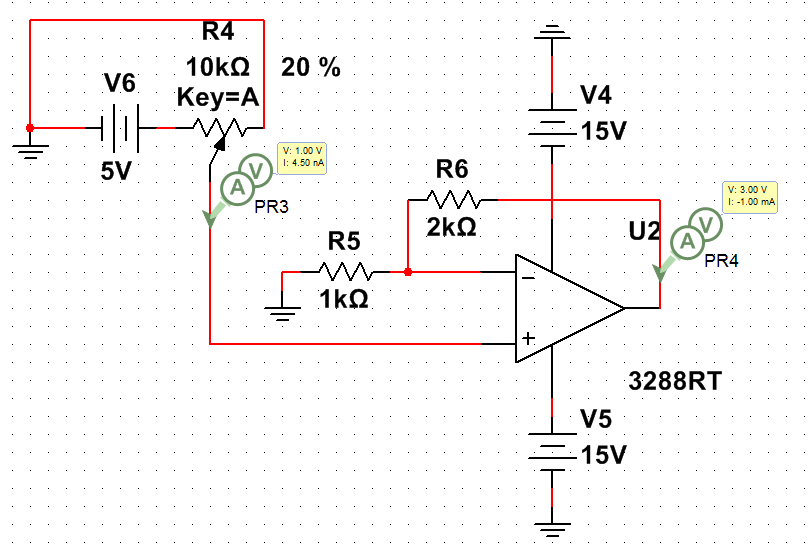
\includegraphics[width=5.5in]{non_inverting_multisim.PNG} 
   \caption{Non-Inverting Amplifier (Multisim)}
   \label{fig:example}
\end{figure}

\bigskip

\begin{figure}[h!] %  figure placement: here, top, bottom, or page
   \centering
   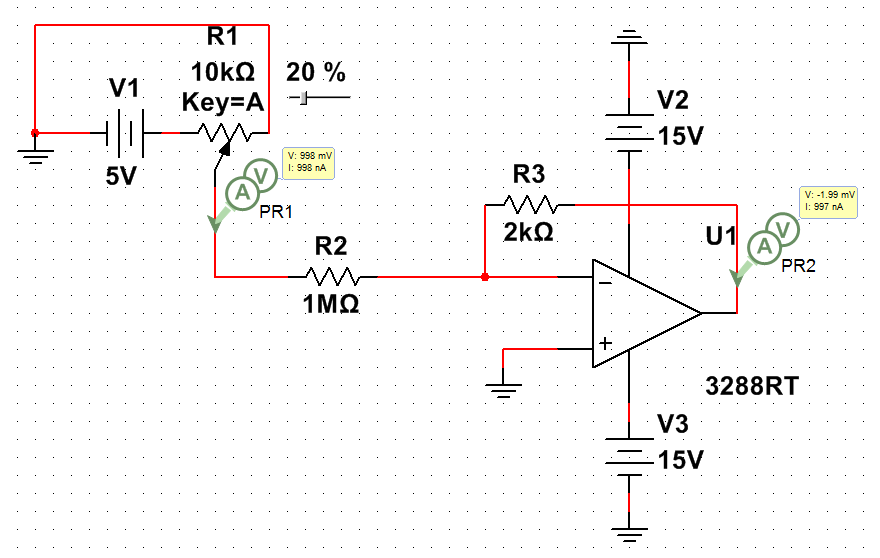
\includegraphics[width=5in]{inverting_multisim.PNG} 
   \caption{Inverting Amplifier (Multisim)}
   \label{fig:example}
\end{figure}

\newpage

\begin{figure}[h!] %  figure placement: here, top, bottom, or page
   \centering
   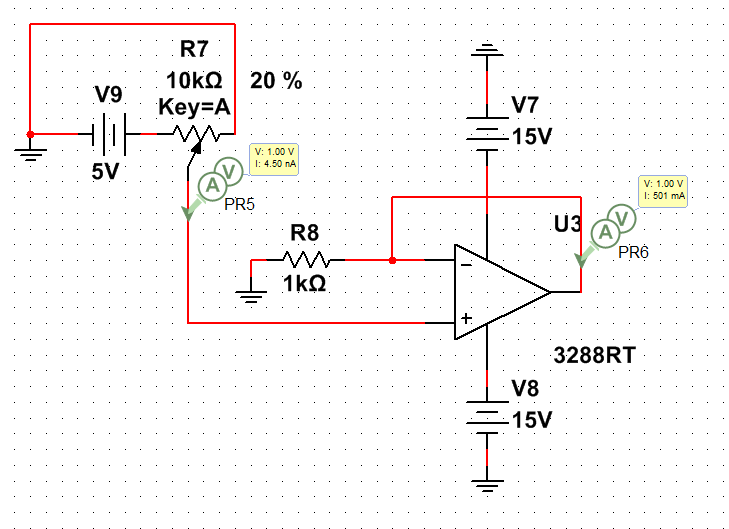
\includegraphics[width=4.5in]{follower_multisim.PNG} 
   \caption{Follower Device (Signal Buffer) (Multisim)}
   \label{fig:example}
\end{figure}

\bigskip

These circuits were then recreated physically in the lab. The input voltage to the circuit was measured and tabulated, as well as the resistances $R_{1}$ and $R_{2}$. The gain for each circuit was calculated using the nominal and measured resistance values with Equations 1 and 2. The predicted output voltages were also calculated using Equations 1 and 2.  The physical implementations of the inverting, non-inverting, and follower circuits can be seen in Figures 4 - 6. The tabulated and calculated data is shown in Figure 7.
\bigskip


% Lab figures
\begin{figure}[h!] %  figure placement: here, top, bottom, or page
   \centering
   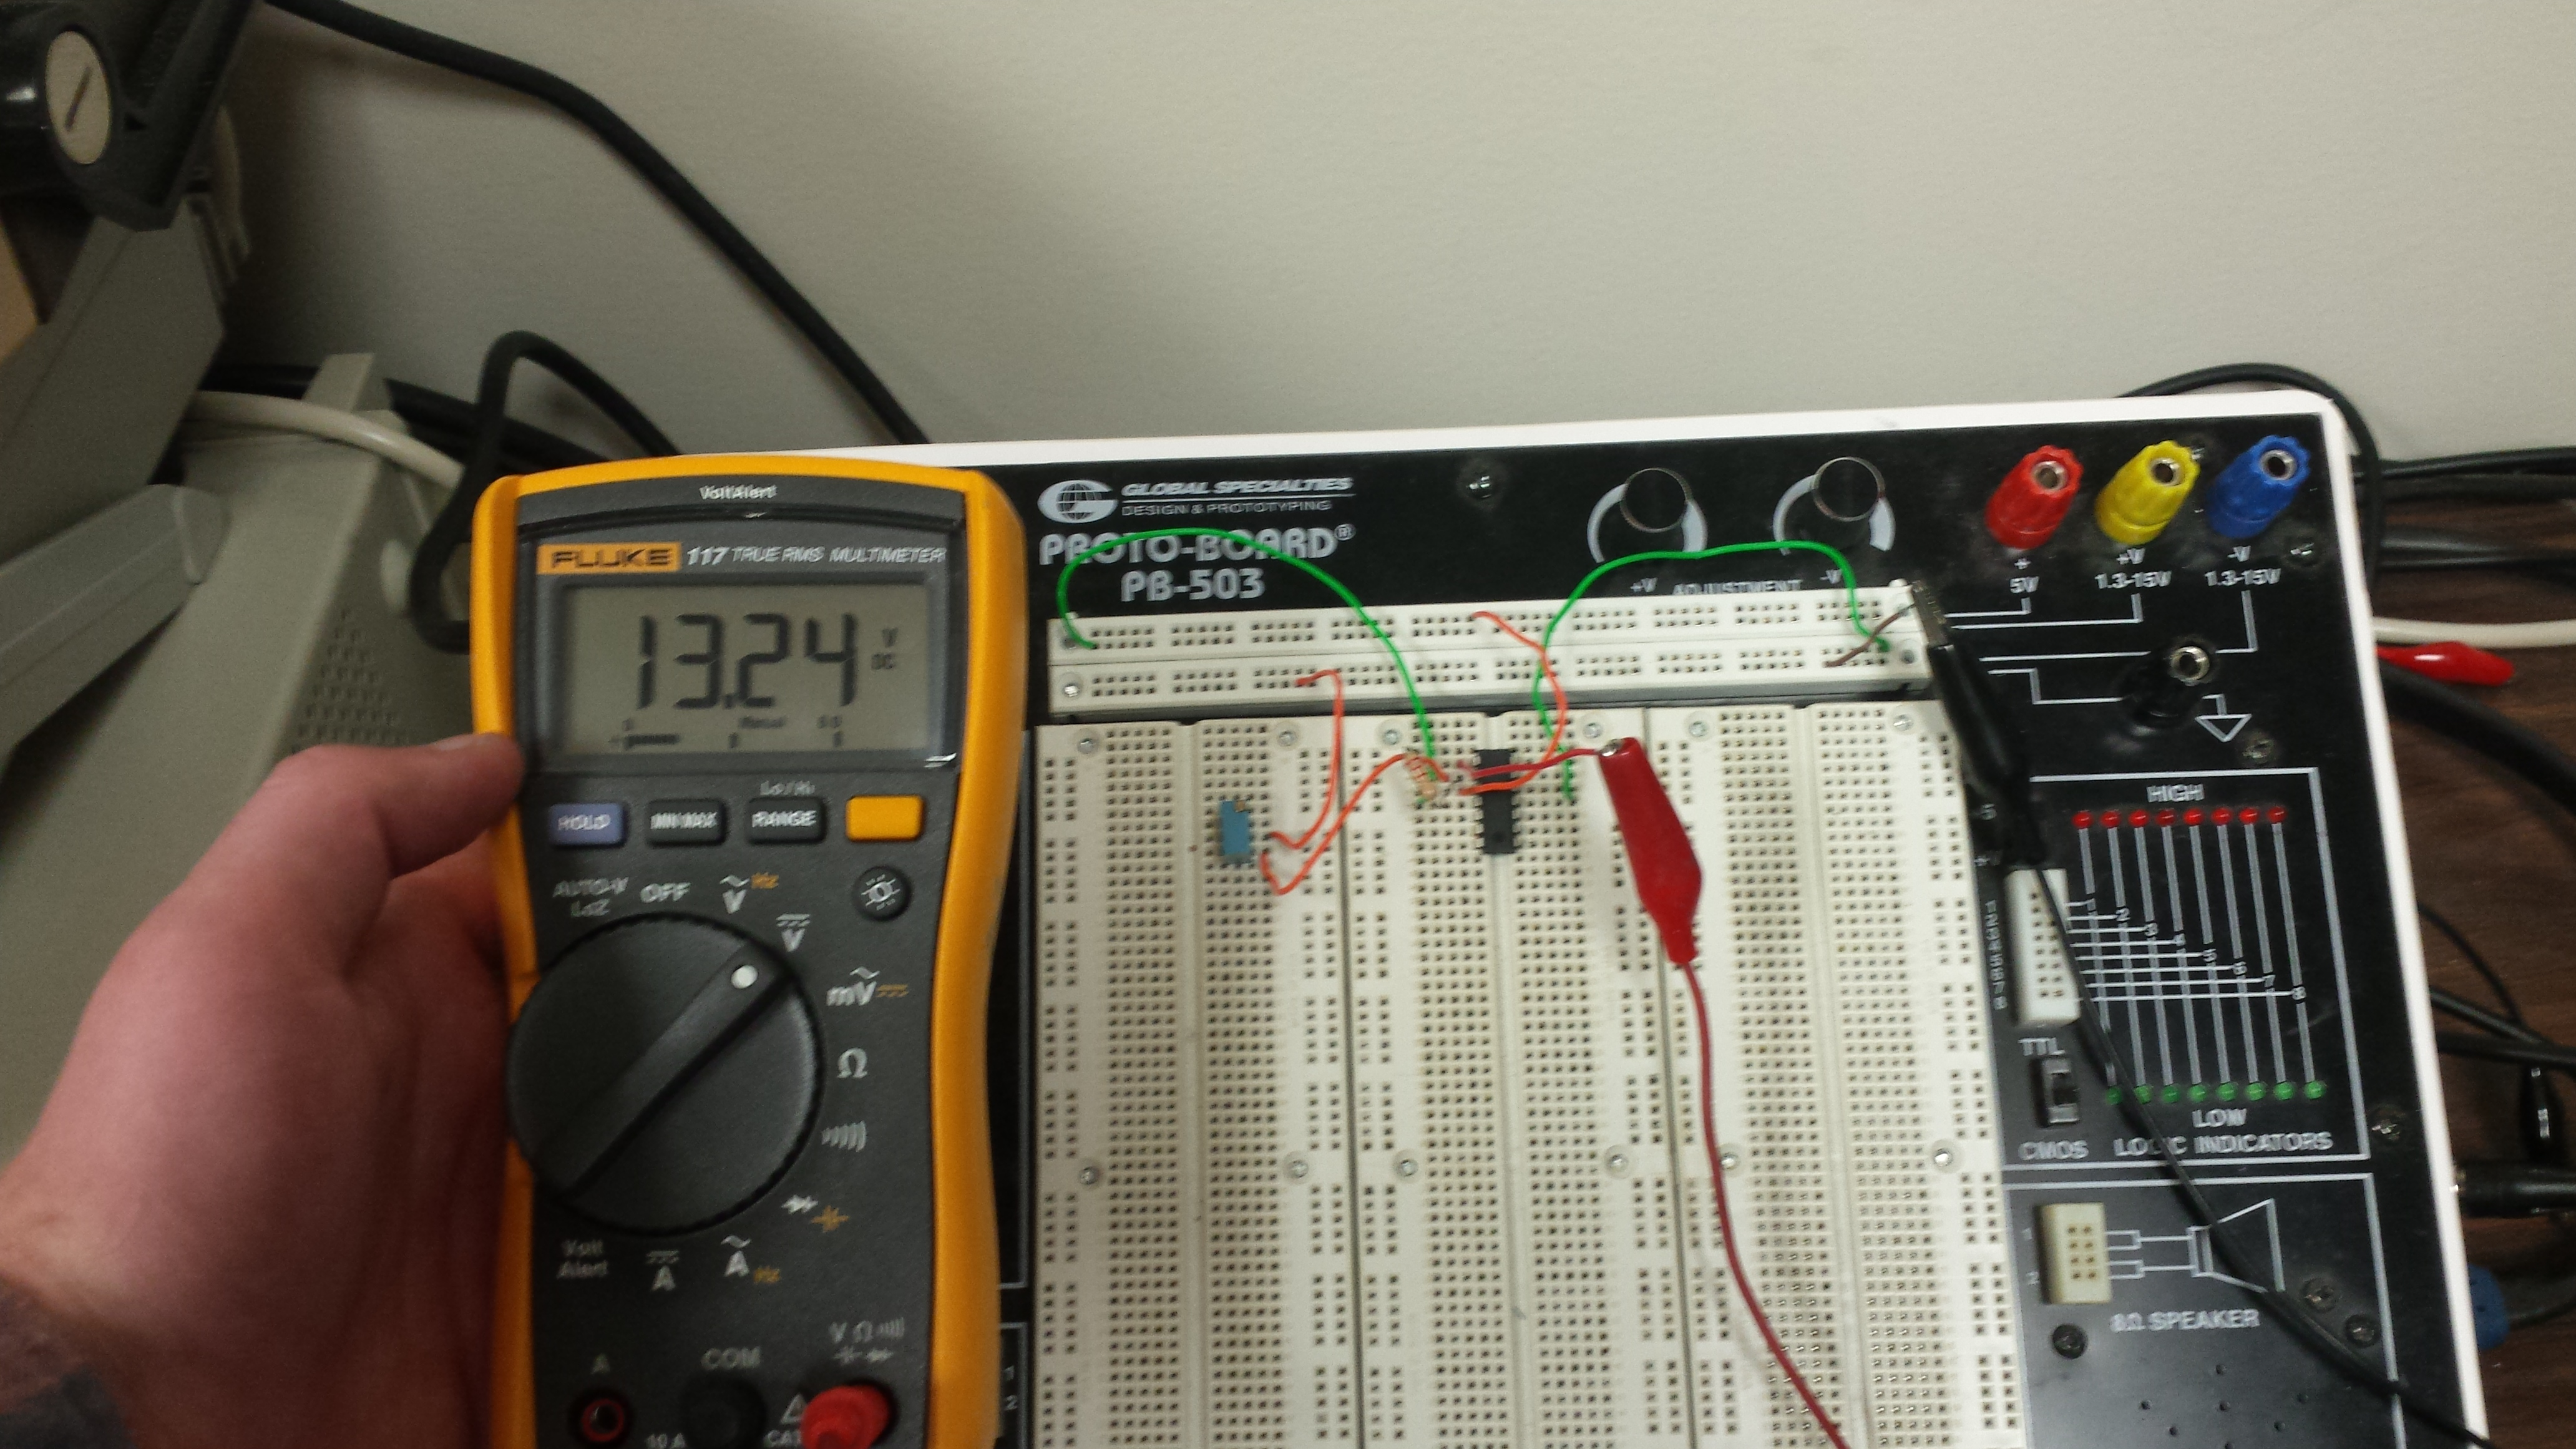
\includegraphics[width=5.5in]{non_inverting_physical.jpg} 
   \caption{Non-Inverting Amplifier (Physical)}
   \label{fig:example}
\end{figure}

\newpage

\begin{figure}[h!] %  figure placement: here, top, bottom, or page
   \centering
   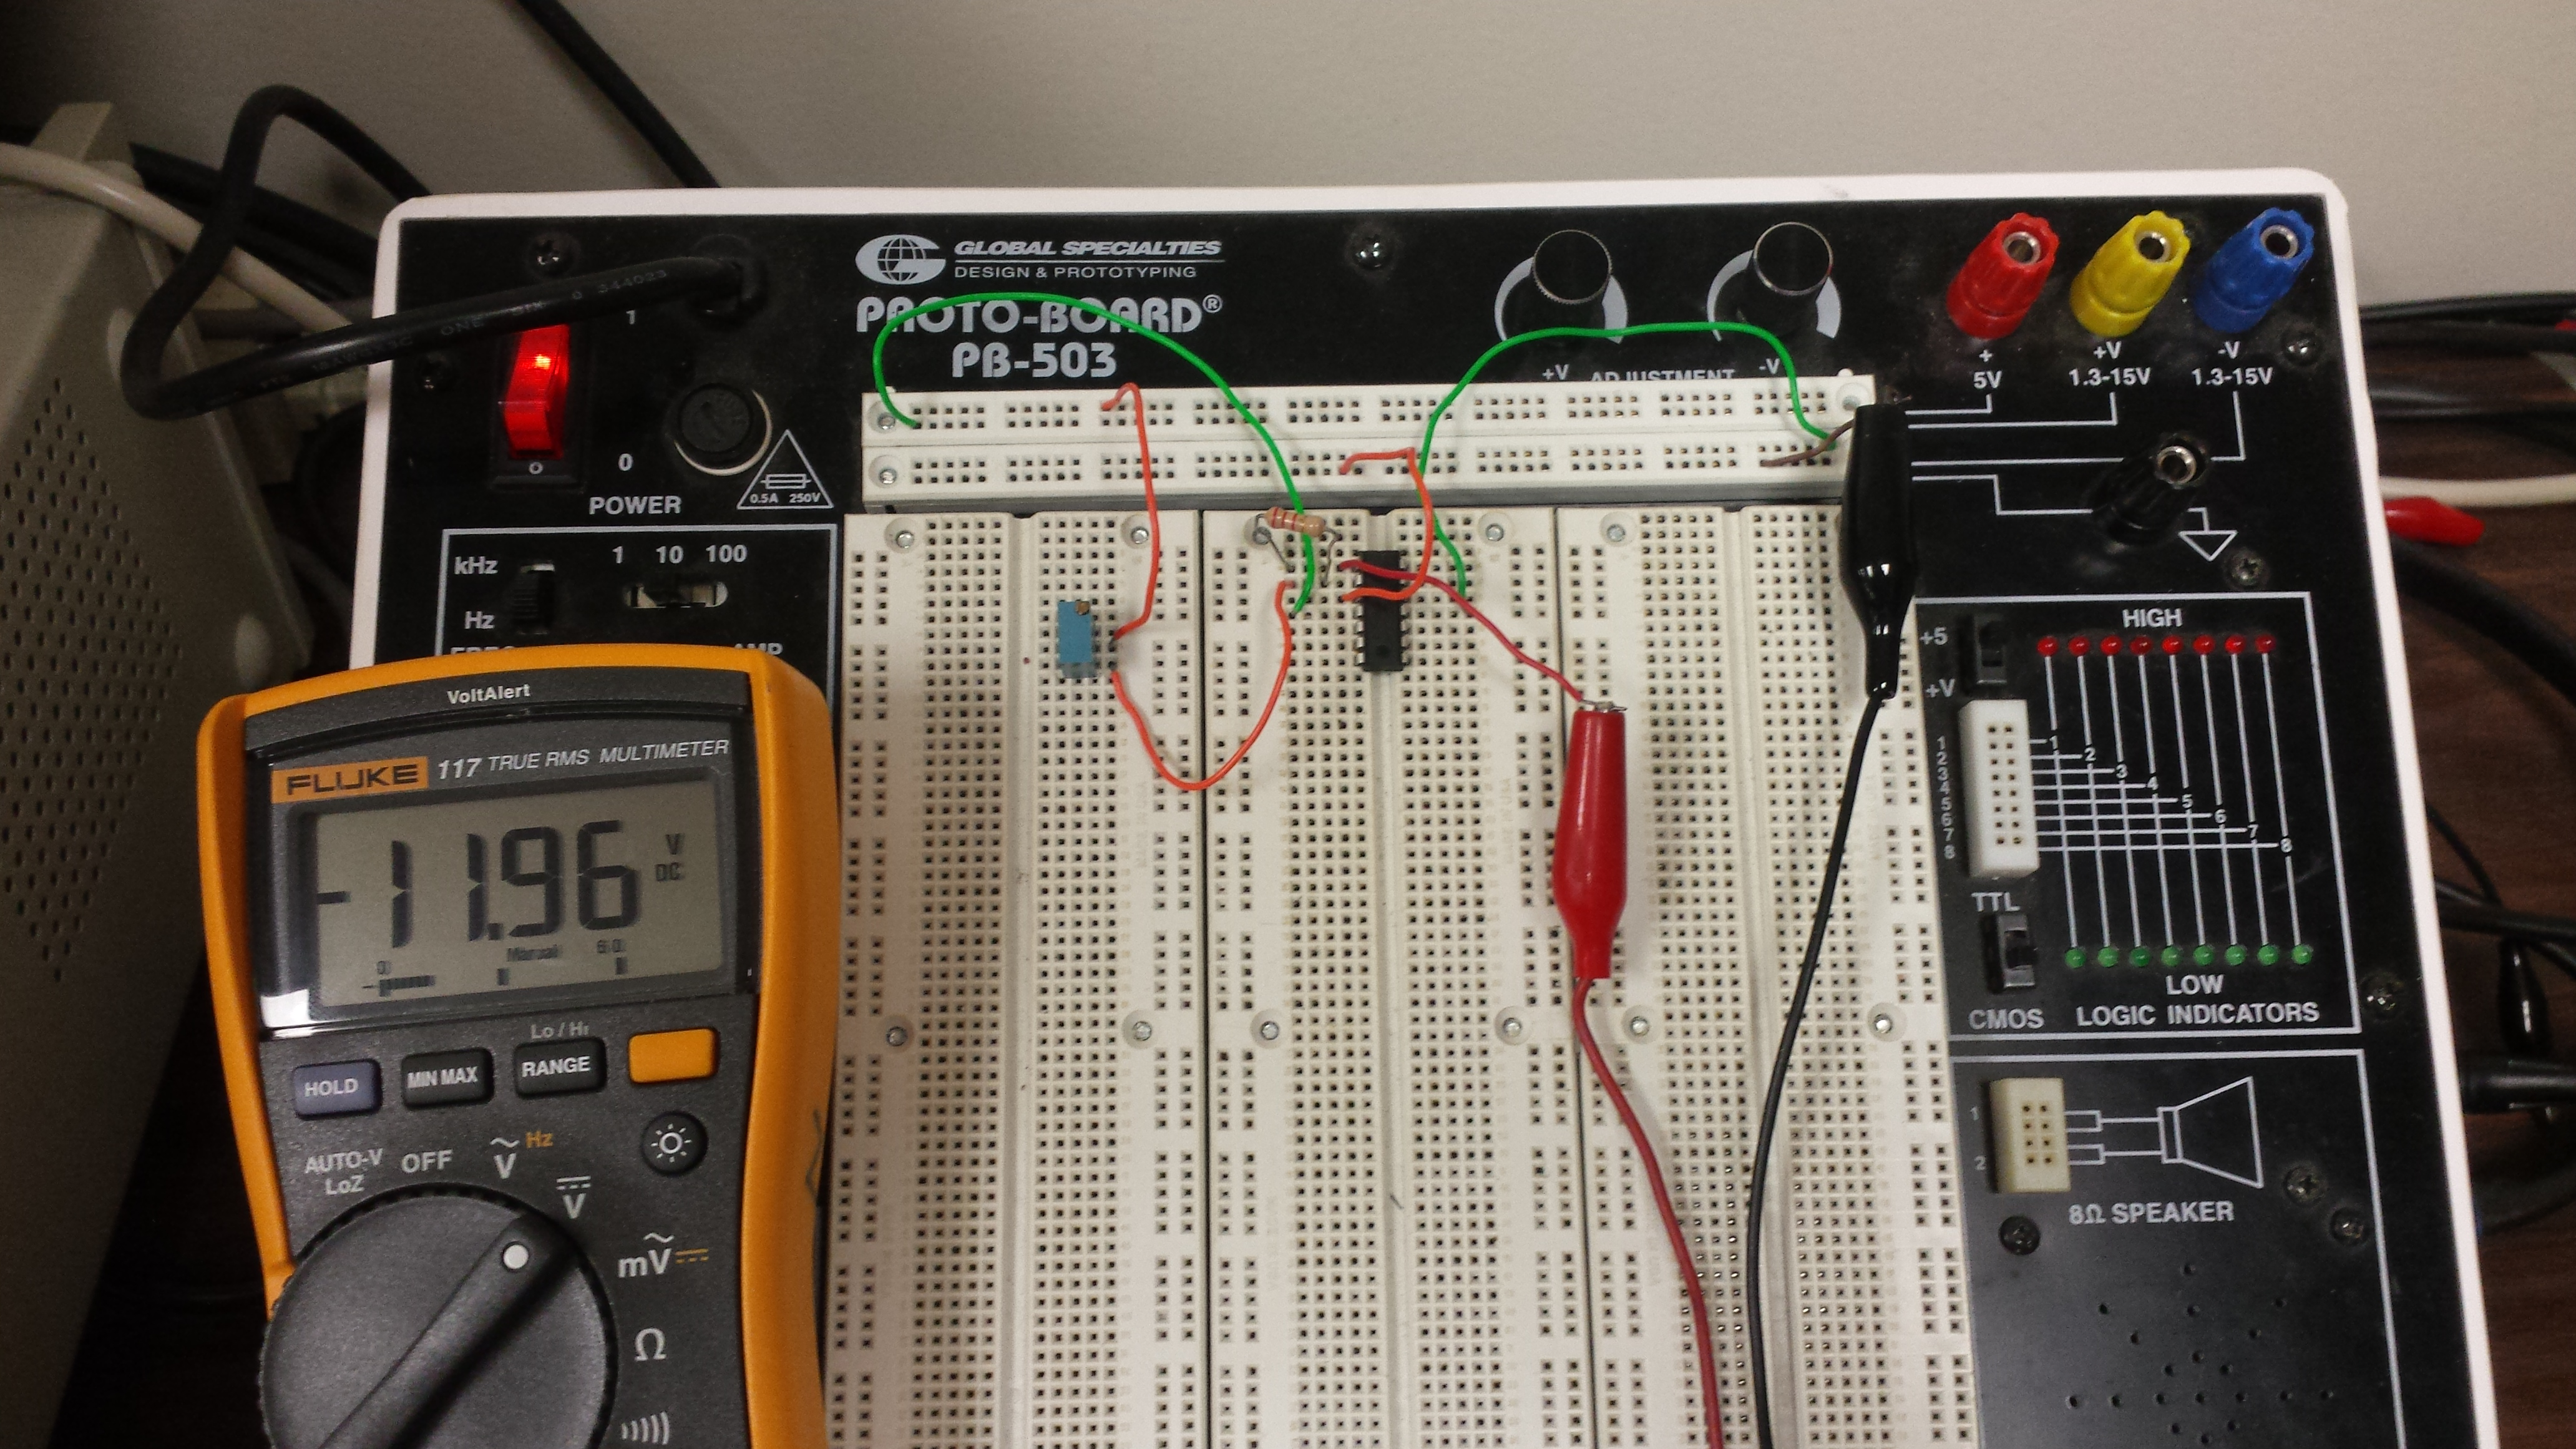
\includegraphics[width=\linewidth]{inverting_physical.jpg} 
   \caption{Inverting Amplifier (Physical)}
   \label{fig:example}
\end{figure}
\bigskip

\begin{figure}[h!] %  figure placement: here, top, bottom, or page
   \centering
   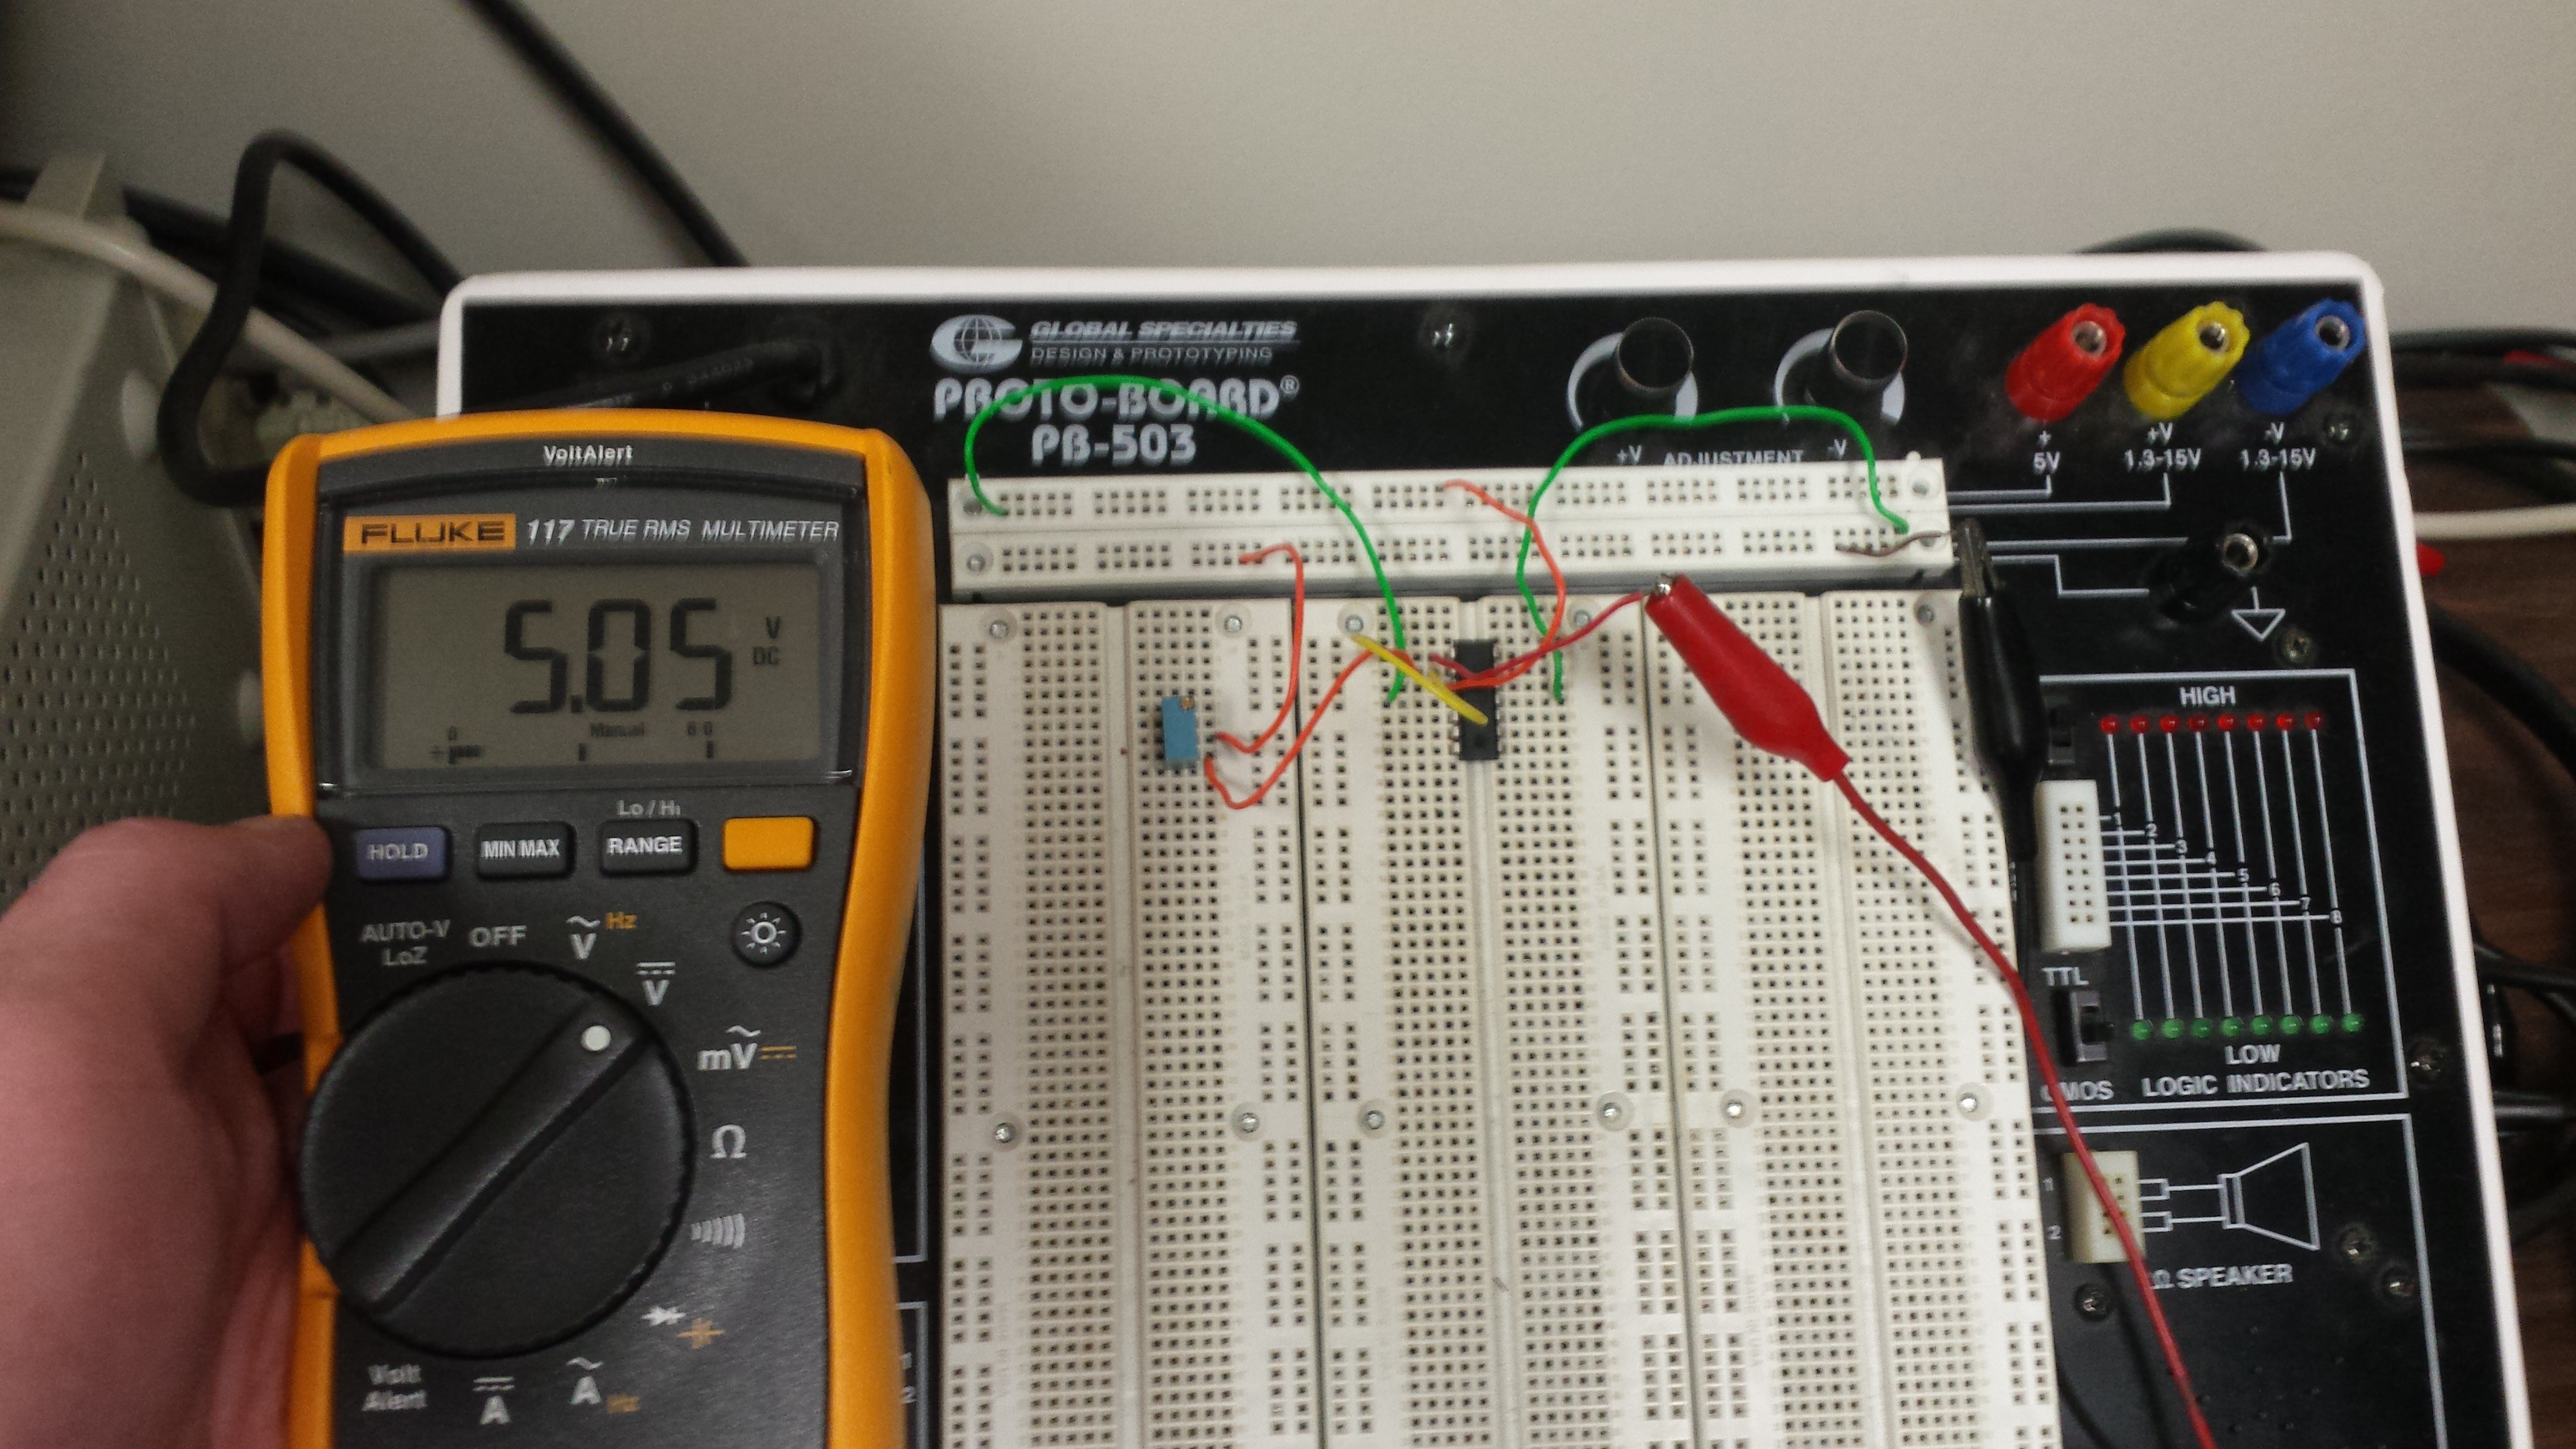
\includegraphics[width=\linewidth]{follower_physical.jpg} 
   \caption{Follower Device (Signal Buffer) (Physical)}
   \label{fig:example}
\end{figure}

\newpage

\begin{figure}[htbp] %  figure placement: here, top, bottom, or page
   \centering
   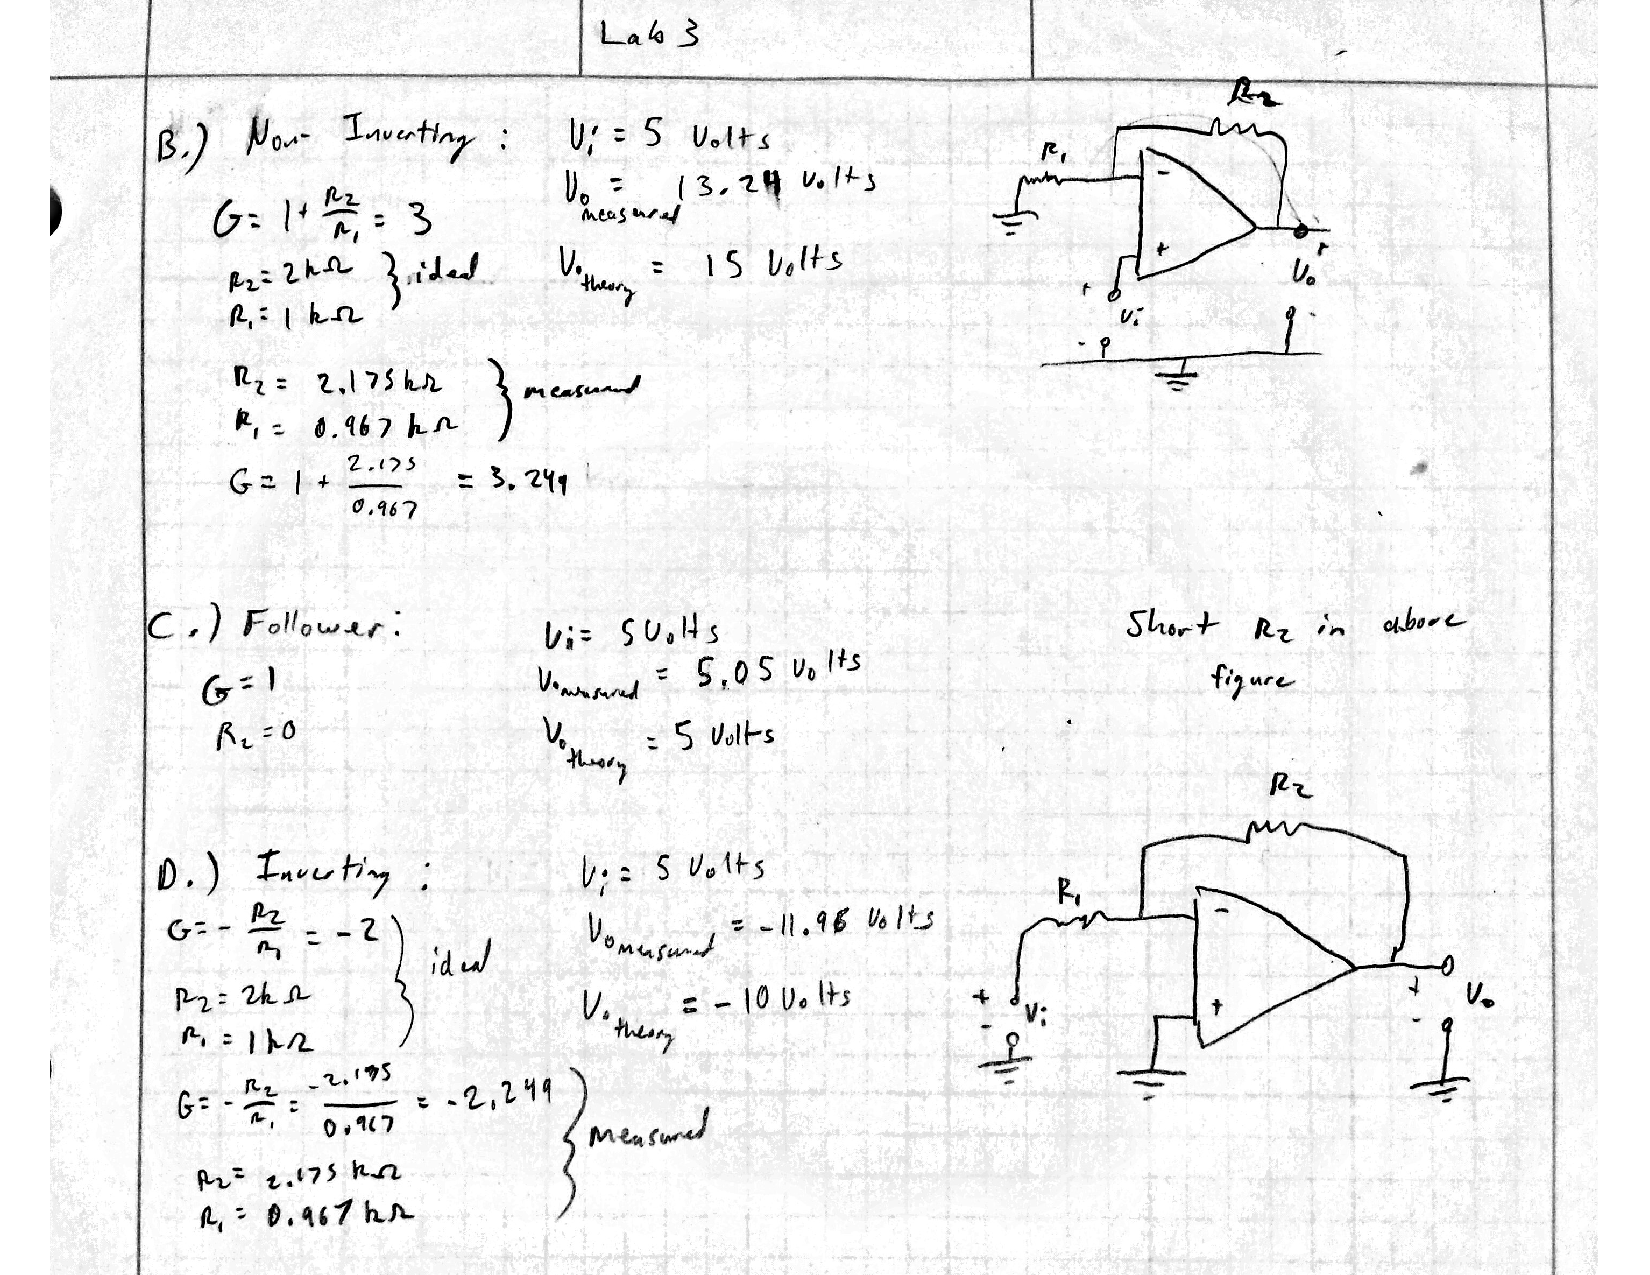
\includegraphics[width=\linewidth]{lab_calculations.pdf} 
   \caption{Tabulated Data \& Calculations (Physical)}
   \label{fig:example}
\end{figure}
\bigskip



\section*{\fontsize{12}{12}\selectfont \large Conclusion}
\addcontentsline{toc}{section}{Conclusion} % Add for each section
The exercises conducted in this lab reinforce the theory learned in the classroom. It is shown that electric circuits can be modeled and analyzed in Multisim. The circuits created in this lab are commonplace in electronic circuits, and the creation of these circuits in Multisim helps the student to further understand what is really happening in these circuits. The first hand experience physically building these circuits in the lab supplements the information previously learned about amplifiers, and is very beneficial.


%\section*{\fontsize{12}{12}\selectfont \large References}

\begin{thebibliography}{2}

% Example
%\bibitem{Wagner}
%Ng, K., Wagner, S.W., Camelio, J., Emblom, W.J. (2010). ?Experimental Analysis of Micro Tube
%Hydroforming Process.? Transactions of NAMRC of SME, 38, 577-584.

\end{thebibliography}



%\section*{\fontsize{12}{12}\selectfont APPENDIX}

%\begin{table}[h!]
%  \caption{}
%  \includegraphics[width=\linewidth]{table1.png}
%\end{table}




\end{document}







----------------------------Templates-------------------------------

-------------------------Figure-----------------------

\begin{figure}[h!]  
  \centering
    \includegraphics[width=\linewidth]{**file**}
    \caption{Docking Station}
\end{figure}

---------------------------Table-----------------------
\begin{table}[ht]
\caption{Nonlinear Model Results} % title of Table
\centering % used for centering table
\begin{tabular}{c c c c} % centered columns (4 columns)
\hline\hline %inserts double horizontal lines
Case & Method\#1 & Method\#2 & Method\#3 \\ [0.5ex] % inserts table
%heading
\hline % inserts single horizontal line
1 & 50 & 837 & 970 \\ % inserting body of the table
2 & 47 & 877 & 230 \\
3 & 31 & 25 & 415 \\
4 & 35 & 144 & 2356 \\
5 & 45 & 300 & 556 \\ [1ex] % [1ex] adds vertical space
\hline %inserts single line
\end{tabular}
\label{table:nonlin} % is used to refer this table in the text
\end{table}



probably best to insert as an image from excel

\bigskip\\
\begin{table}[h!]
  \caption{}
  \includegraphics[width=\linewidth]{**file**}
\end{table}
\bigskip\\





-----------------------------Equations------------------------
-----------------------------Regular
\begin{equation}
a = b + c
\end{equation}

--------------------------------- Multiline
\begin{multline}
a = b + c + d + e + f
+ g + h + i + j \\
+ k + l + m + n + o
\end{multline}

-------------------------------Citations-------------------------
\bibitem{Author last name}
  Last, First., year of publication,
  article name, book(etc) name, from \\
  link goes here

----------------------------------other-----------------------------

equations:
http://moser-isi.ethz.ch/docs/typeset_equations.pdf

citations:
http://library.missouri.edu/engineering/about/guides/asme
https://www.asme.org/shop/proceedings/conference-publications/references